\section{Histograms on the First Run~\label{sec:sodb9_r1_hist}} 
This section exhibits histograms on the first run of 
INC with its task length increasing from 1 second to 4096 seconds, via EMPv5. 
The detailed description of the base data is from Table~\ref{tab:exp_notes1}.

\section{Experiment Notes}
Table~\ref{tab:exp_notes1} provides a short description of our experimental runs, 
on which the following histograms are based.

%% done
\begin{table}[h]
\begin{center}
\begin{tabular}{|p{2cm}|p{3cm}|p{3cm}|p{4cm}|p{3cm}|} \hline
Machine & Task Length (sec) & Description & Experiment Period & Relevant \linebreak Histograms\\ \hline
{\tt sodb9} &  INC1$\sim$INC64 & 1000 samples, each & 2017-03-02 $\sim$ 2017-03-04 & Figs.~\ref{fig:s9_r1_et_hist1},~\ref{fig:s9_r1_et_hist2},~\ref{fig:s9_r1_pt_hist1}, and~\ref{fig:s9_r1_pt_hist2}\\ \hline
{\tt sodb9} &  INC128$\sim$INC1024 & 300 samples, each & 2017-03-04 $\sim$ 2017-03-11 & 
Figs.~\ref{fig:s9_r1_et_hist3} and~\ref{fig:s9_r1_pt_hist3}\\ \hline
{\tt sodb10} & INC2048 & 300 samples & 2017-03-02 $\sim$ 2017-03-09 & Figs.~\ref{fig:inc2048_r1_et_hist_v5} and~\ref{fig:inc2048_r1_hist_v5}\\ \hline
{\tt sodb12} & INC4096 & 300 samples & 2017-02-13 $\sim$ 2017-02-27 & Figs.~\ref{fig:inc4096_r1_et_hist_v5} and~\ref{fig:inc4096_r1_hist_v5}\\ \hline
\end{tabular}
\end{center}
\vspace{-.2in}
\caption{Notes on experiment runs used for histograms\label{tab:exp_notes1}}
\end{table}

\pagebreak

\subsection{ET}

\begin{figure}[hp!]
	\centering
	\subfigure[ET frequency on INC1]{
		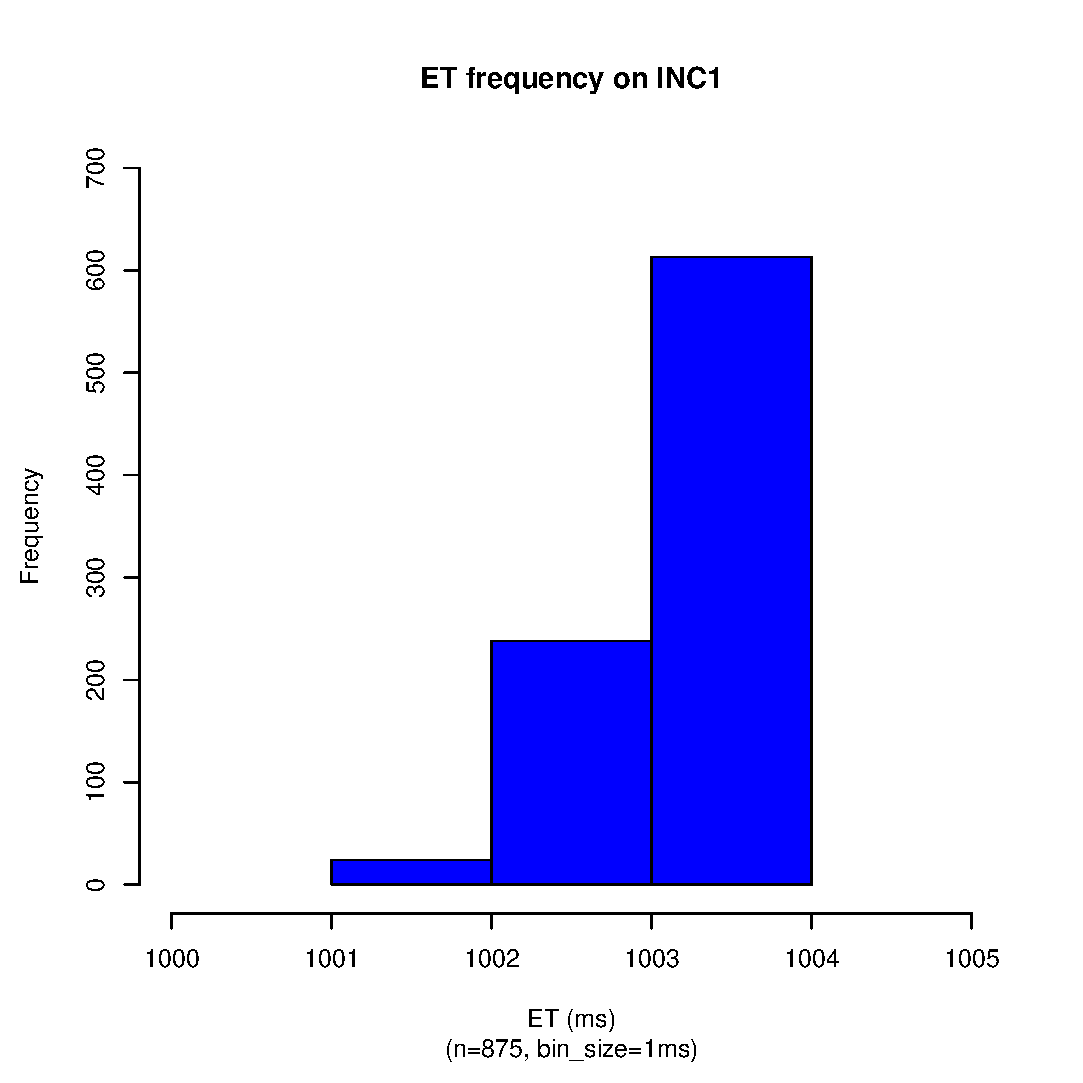
\includegraphics[scale=0.43]{repet_data1/1_sec_et_hist_v5.eps}
		\label{fig:inc1_r1_et_hist_v5}
	}
	\subfigure[ET frequency on INC2]{
		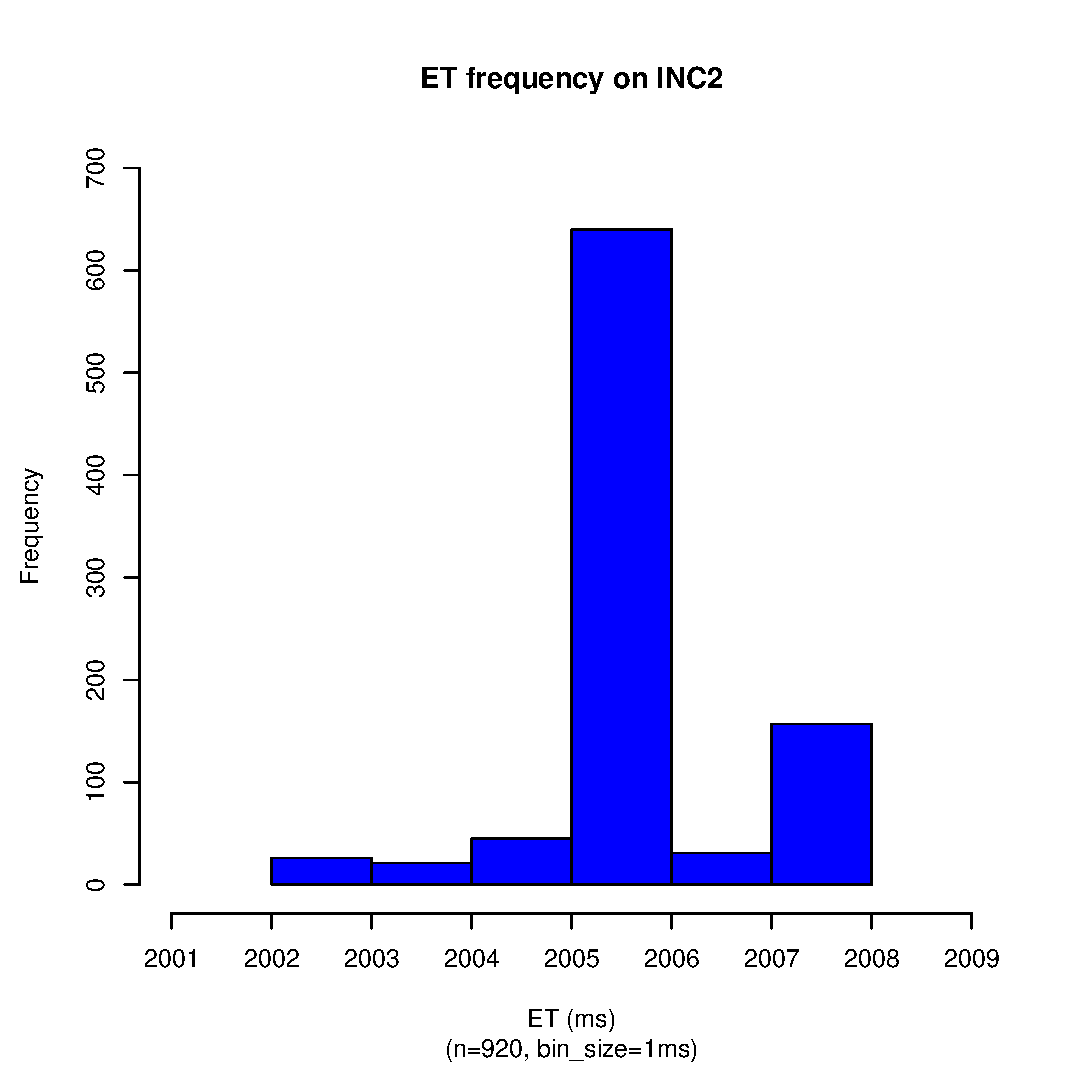
\includegraphics[scale=0.43]{repet_data1/2_sec_et_hist_v5.eps}
		\label{fig:inc2_r1_et_hist_v5}
	}
	\subfigure[ET frequency on INC4]{
		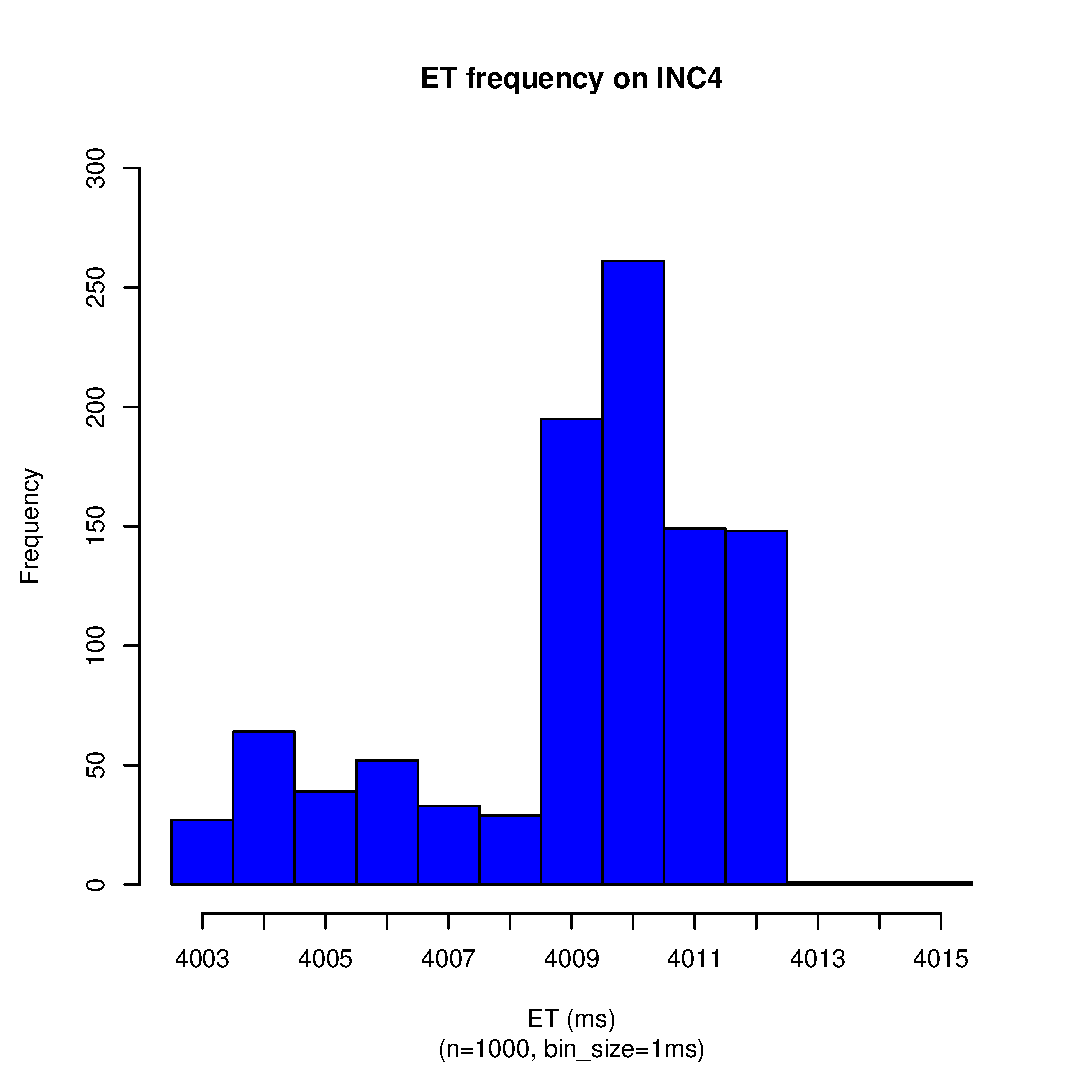
\includegraphics[scale=0.43]{repet_data1/4_sec_et_hist_v5.eps}
		\label{fig:inc4_r1_et_hist_v5}
	}
	\subfigure[ET frequency on INC8]{
		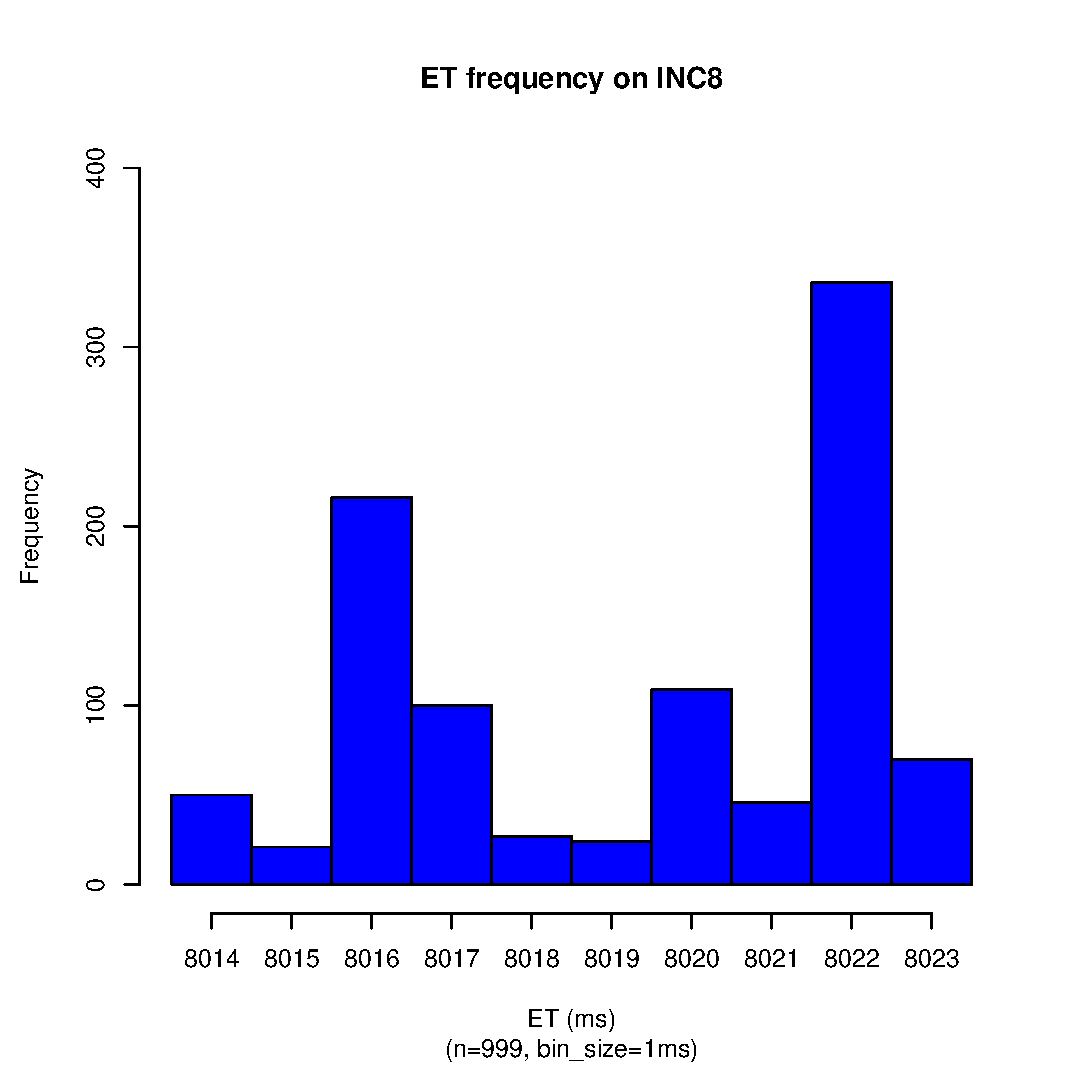
\includegraphics[scale=0.43]{repet_data1/8_sec_et_hist_v5.eps}
		\label{fig:inc8_r1_et_hist_v5}
	}
	\caption{ET Histograms of INC1 ... INC8~\label{fig:s9_r1_et_hist1}}
\end{figure}

\begin{figure}[hp!]
	\centering
	\subfigure[ET frequency on INC16]{
		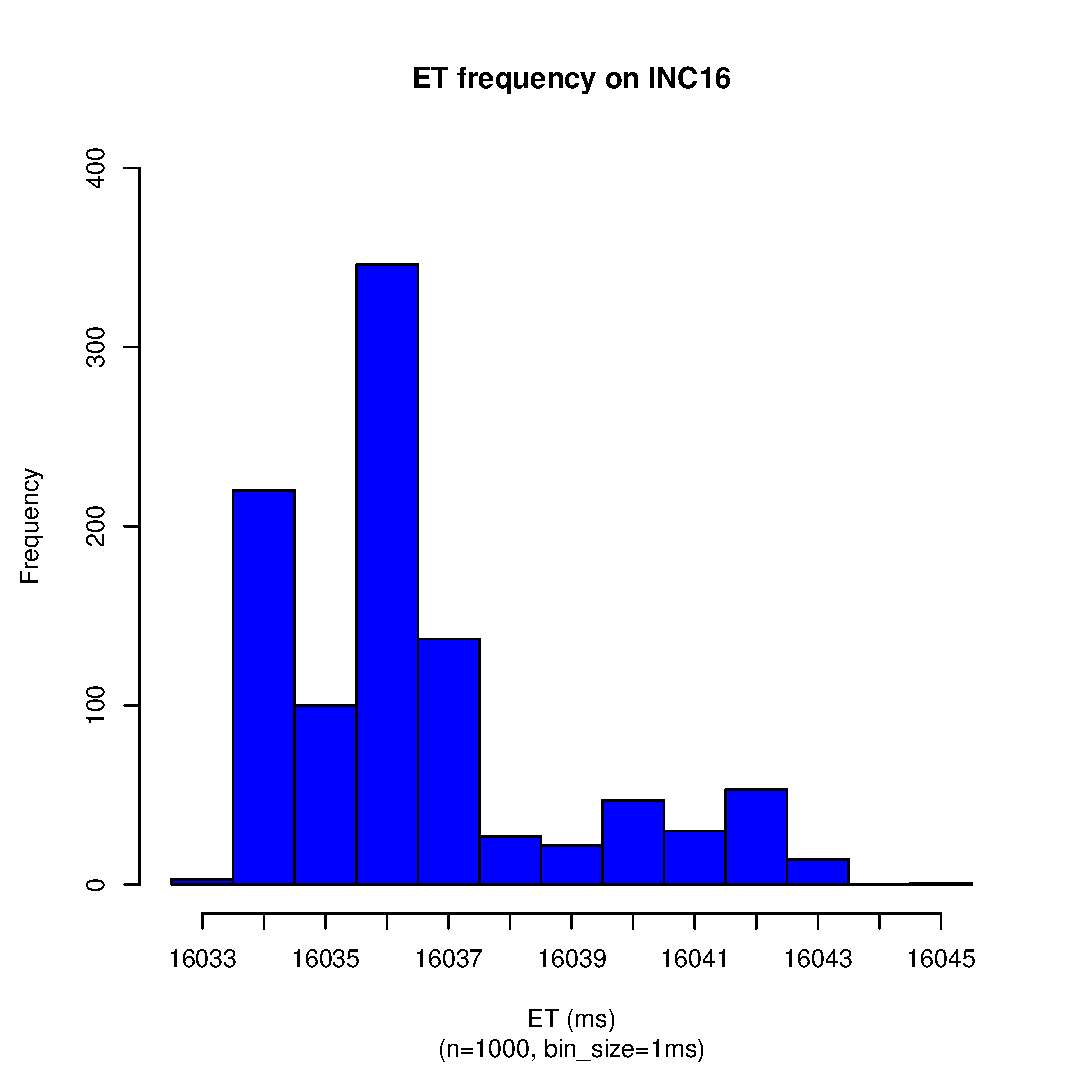
\includegraphics[scale=0.43]{repet_data1/16_sec_et_hist_v5.eps}
		\label{fig:inc16_r1_et_hist_v5}
	}
	\subfigure[ET frequency on INC32]{
		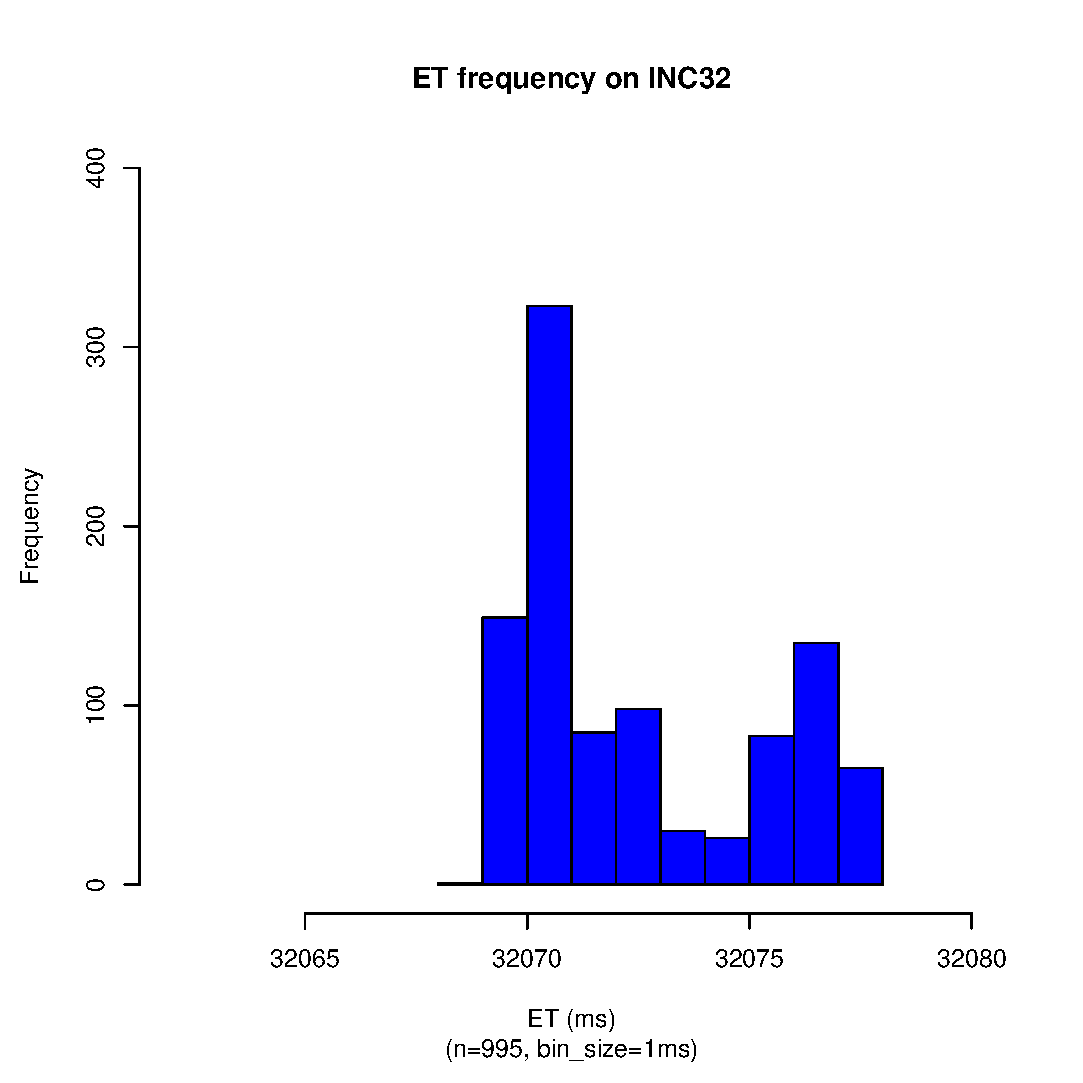
\includegraphics[scale=0.43]{repet_data1/32_sec_et_hist_v5.eps}
		\label{fig:inc32_r1_et_hist_v5}
	}
	\subfigure[ET frequency on INC64]{
		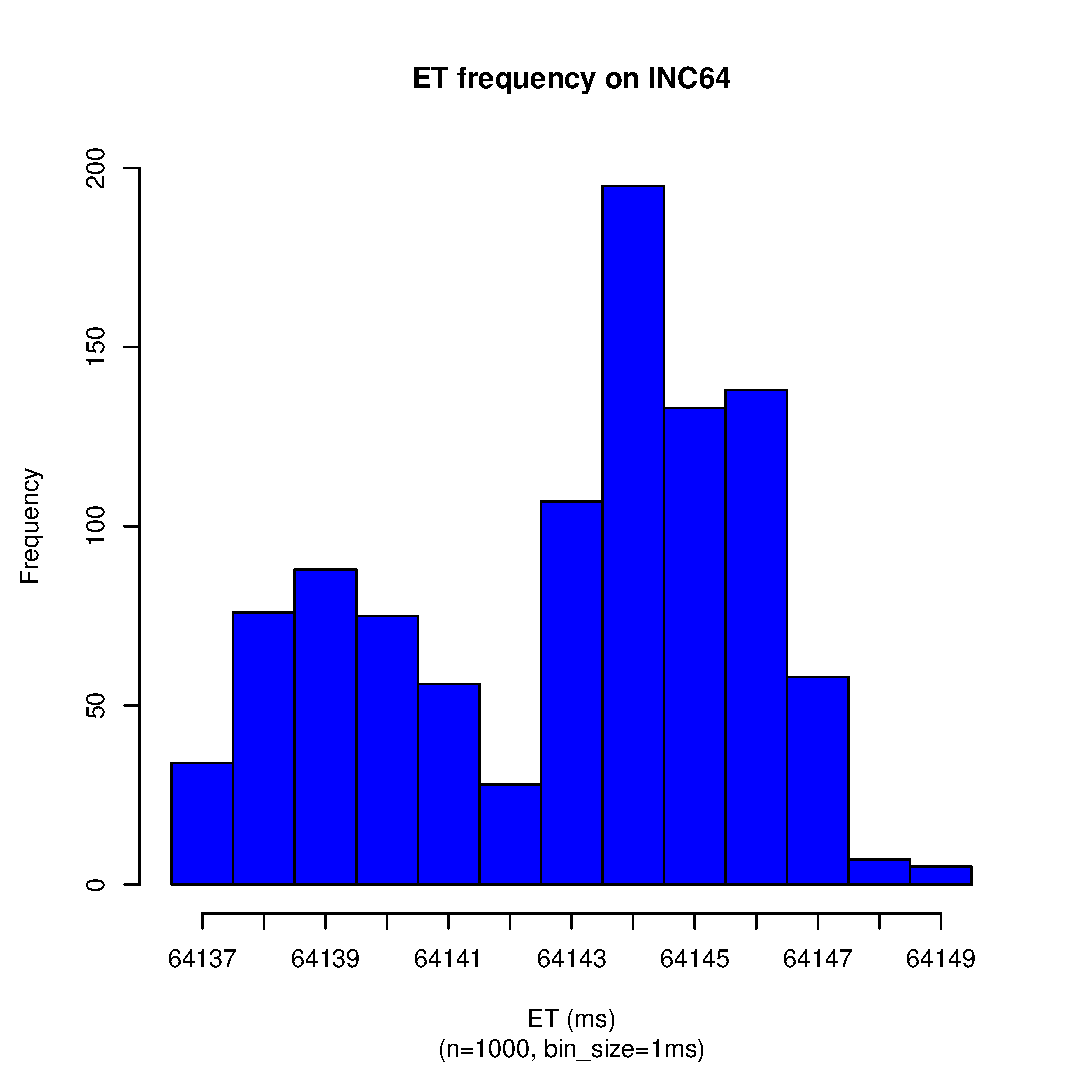
\includegraphics[scale=0.43]{repet_data1/64_sec_et_hist_v5.eps}
		\label{fig:inc64_r1_et_hist_v5}
	}
	\caption{ET Histograms of INC16 ... INC64~\label{fig:s9_r1_et_hist2}}
\end{figure}

\begin{figure}[hp!]
	\centering
	\subfigure[ET frequency on INC128]{
		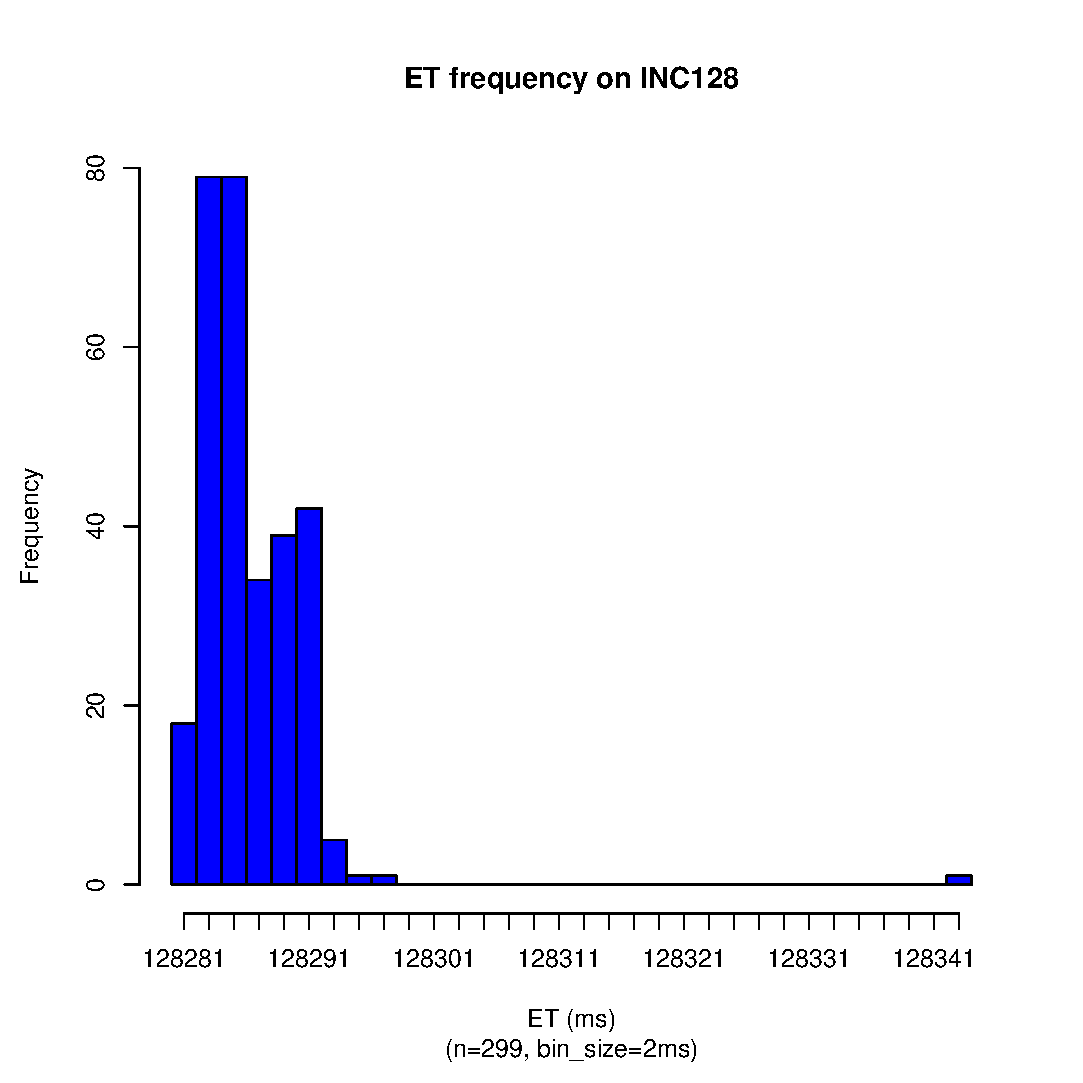
\includegraphics[scale=0.43]{repet_data1/128_sec_et_hist_v5.eps}
		\label{fig:inc128_r1_et_hist_v5}
	}
	\subfigure[ET frequency on INC256]{
		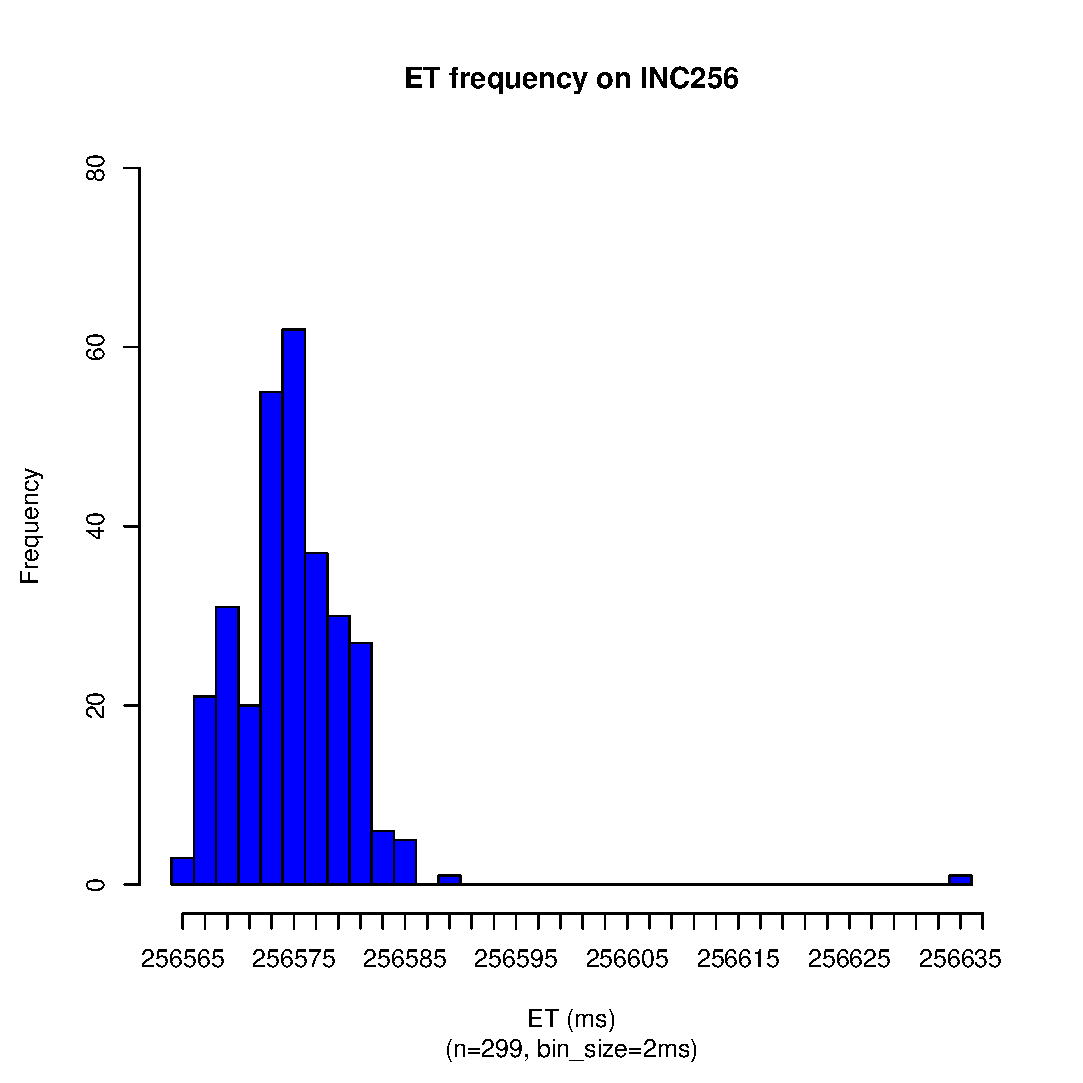
\includegraphics[scale=0.43]{repet_data1/256_sec_et_hist_v5.eps}
		\label{fig:inc256_r1_et_hist_v5}
	}
	\subfigure[ET frequency on INC512]{
		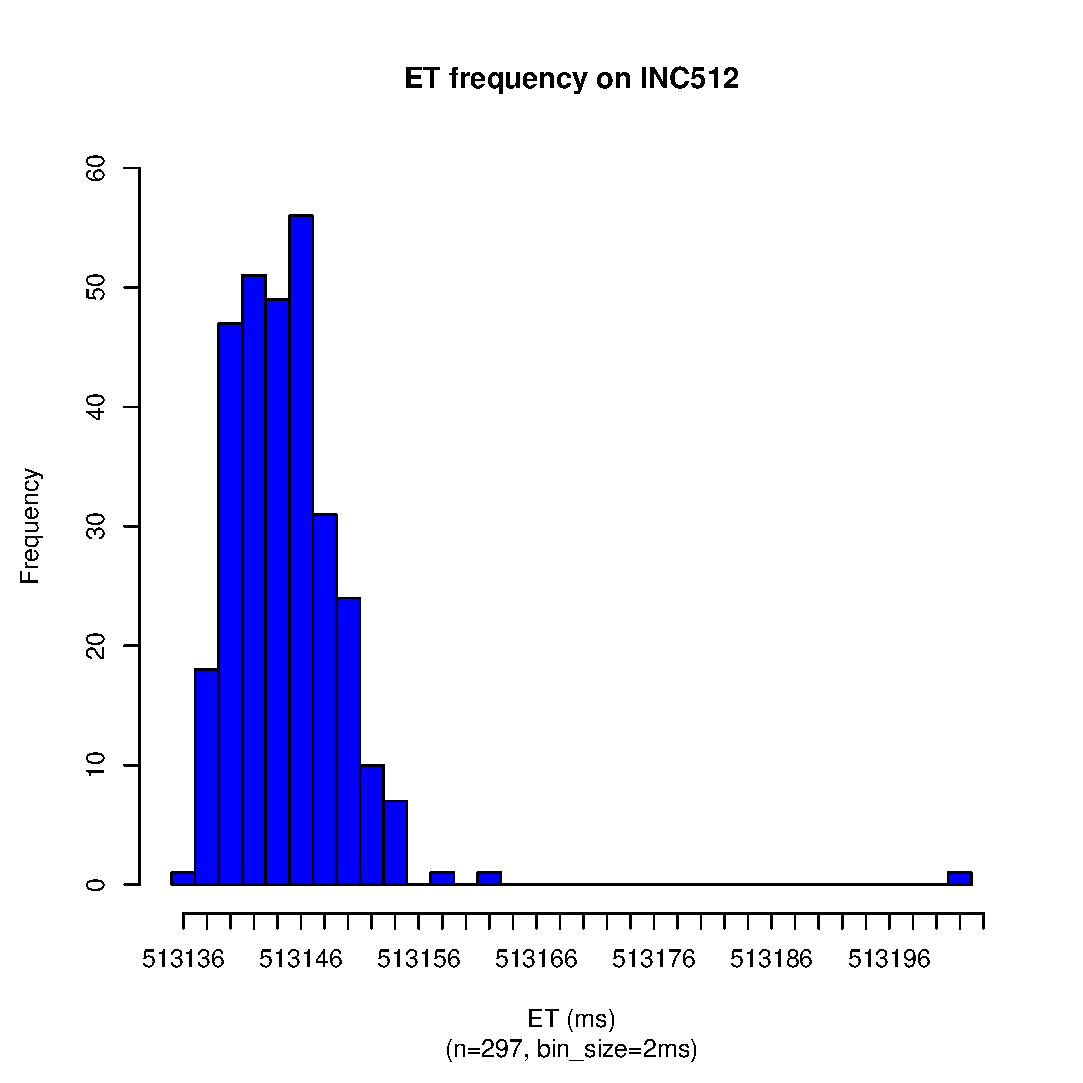
\includegraphics[scale=0.43]{repet_data1/512_sec_et_hist_v5.eps}
		\label{fig:inc512_r1_et_hist_v5}
	}
	\subfigure[ET frequency on INC1024]{
		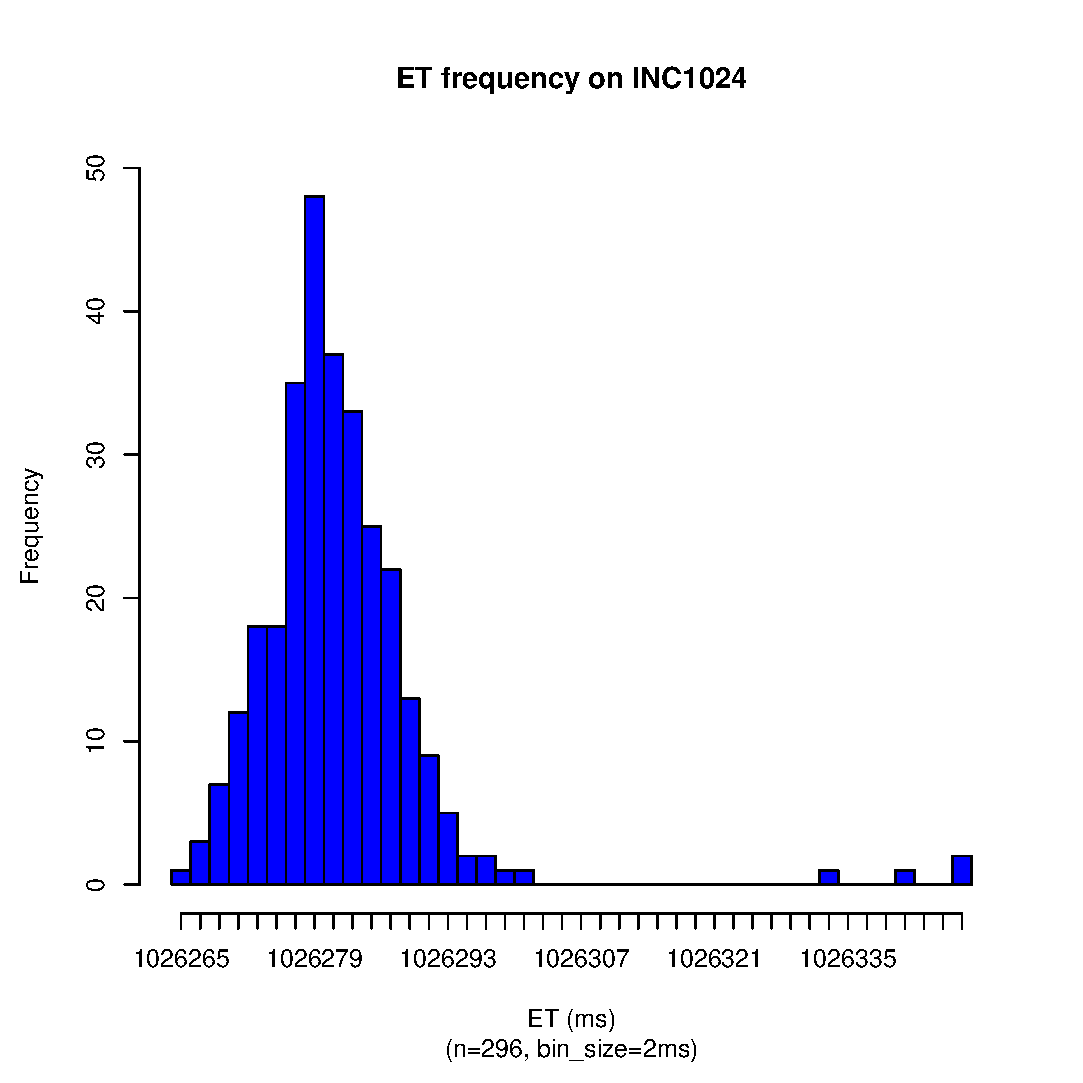
\includegraphics[scale=0.43]{repet_data1/1024_sec_et_hist_v5.eps}
		\label{fig:inc1024_r1_et_hist_v5}
	}
	\caption{ET Histograms of INC128 ... INC1024~\label{fig:s9_r1_et_hist3}}
\end{figure}

\pagebreak

\begin{figure}[t]
	\centering
	\subfigure[ET frequency on INC2048]{
		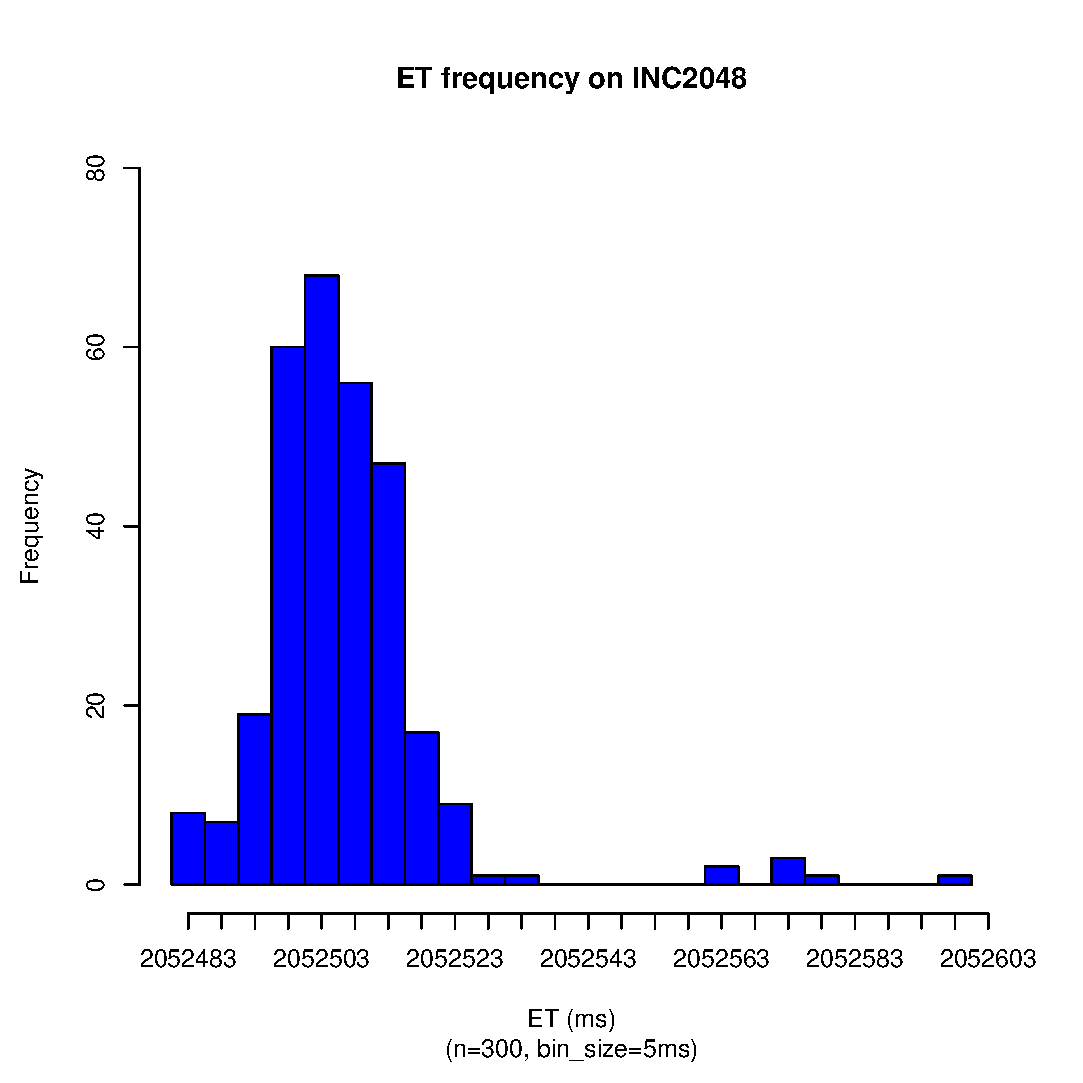
\includegraphics[scale=0.43]{repet_data1/2048_sec_et_hist_v5.eps}
		\label{fig:inc2048_r1_et_hist_v5}
	}
	\subfigure[ET frequency on INC4096]{
		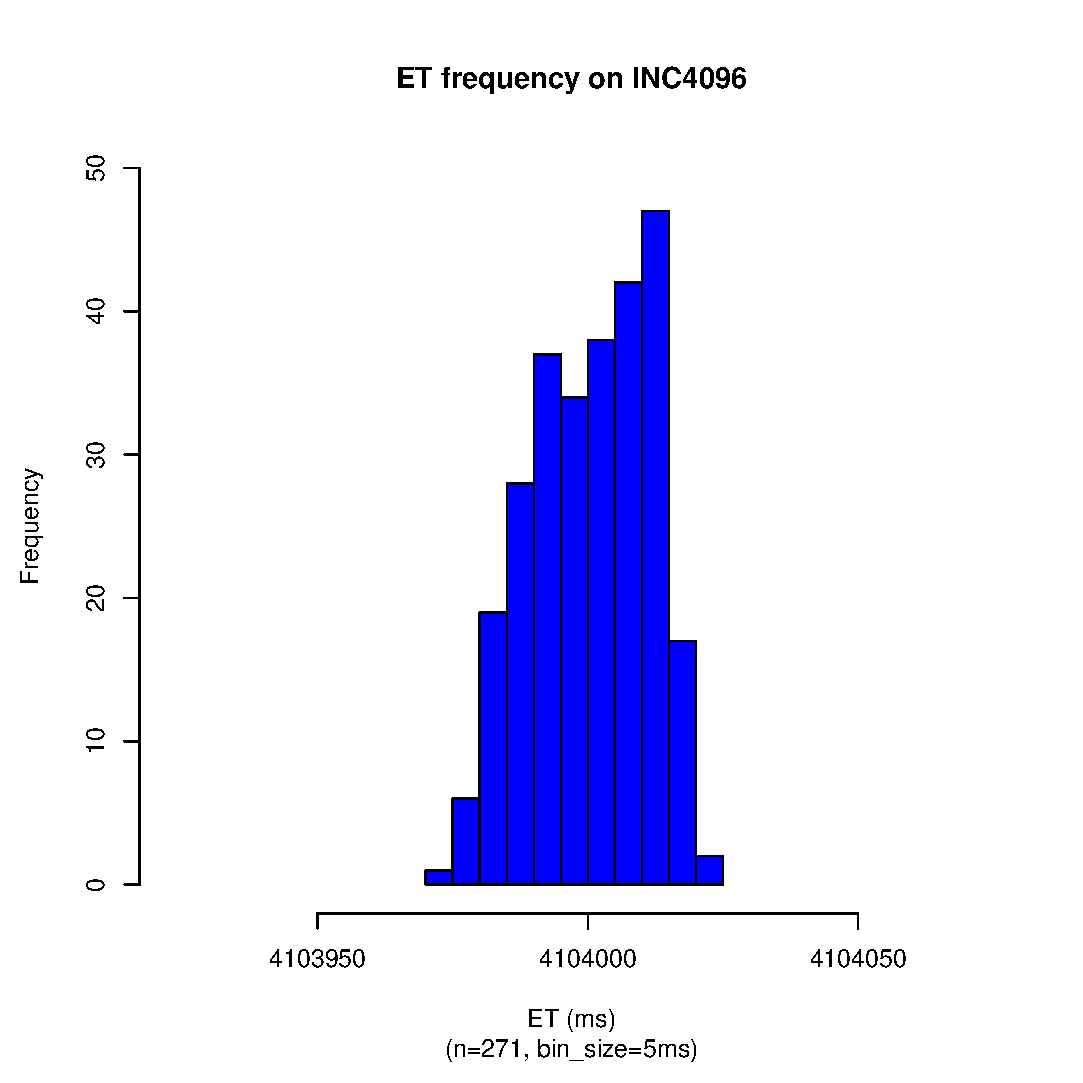
\includegraphics[scale=0.43]{repet_data1/4096_sec_et_hist_v5.eps}
		\label{fig:inc4096_r1_et_hist_v5}
	}
	\caption{ET Histograms of INC2048 and INC4096~\label{fig:s9_r1_et_hist4}}
\end{figure}

\vspace\fill
\clearpage

\subsection{PT}

\begin{figure}[hp!]
	\centering
	\subfigure[PT frequency on INC1]{
		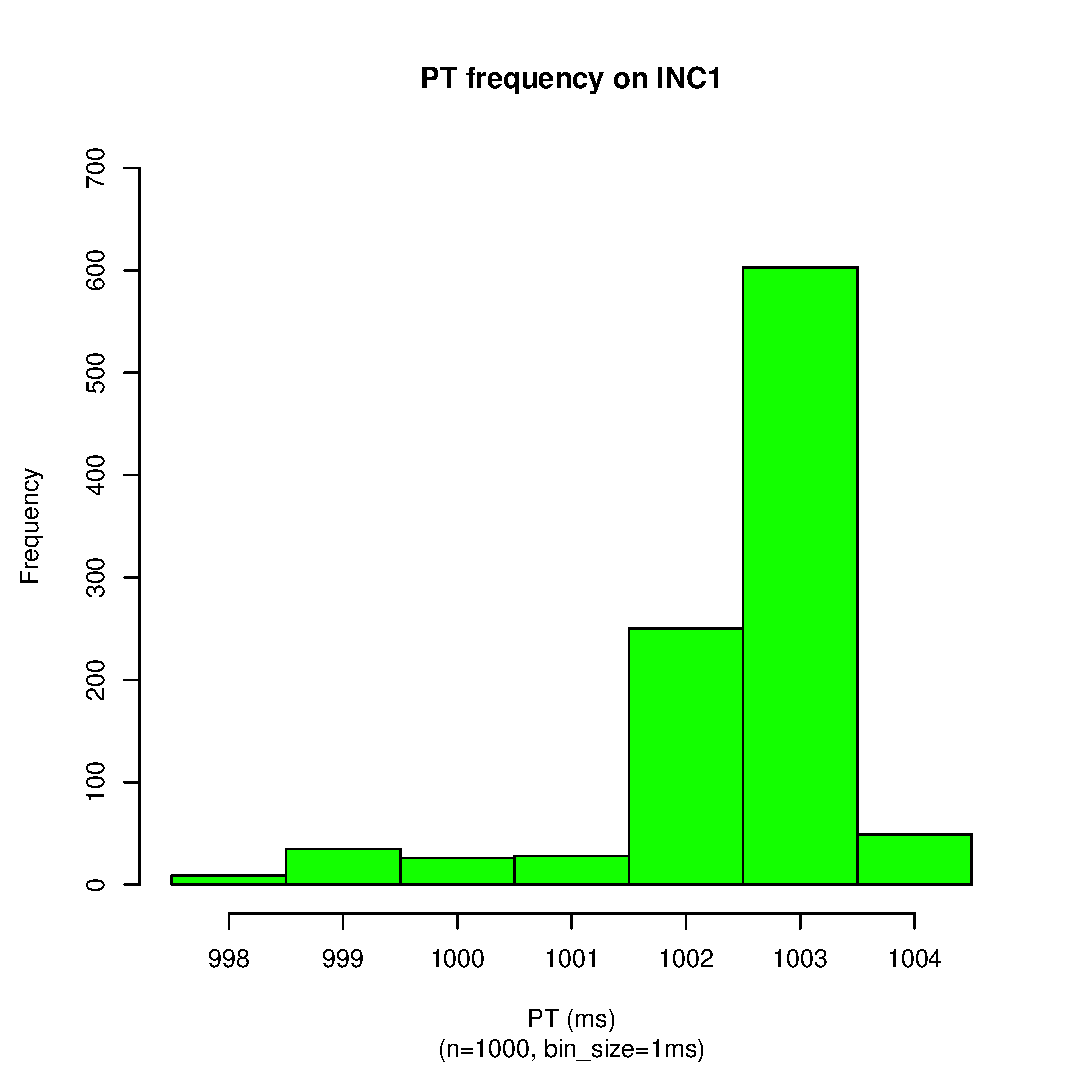
\includegraphics[scale=0.43]{repet_data1/1_sec_pt_hist_v5.eps}
		\label{fig:inc1_r1_hist_v5}
	}
	\subfigure[PT frequency on INC2]{
		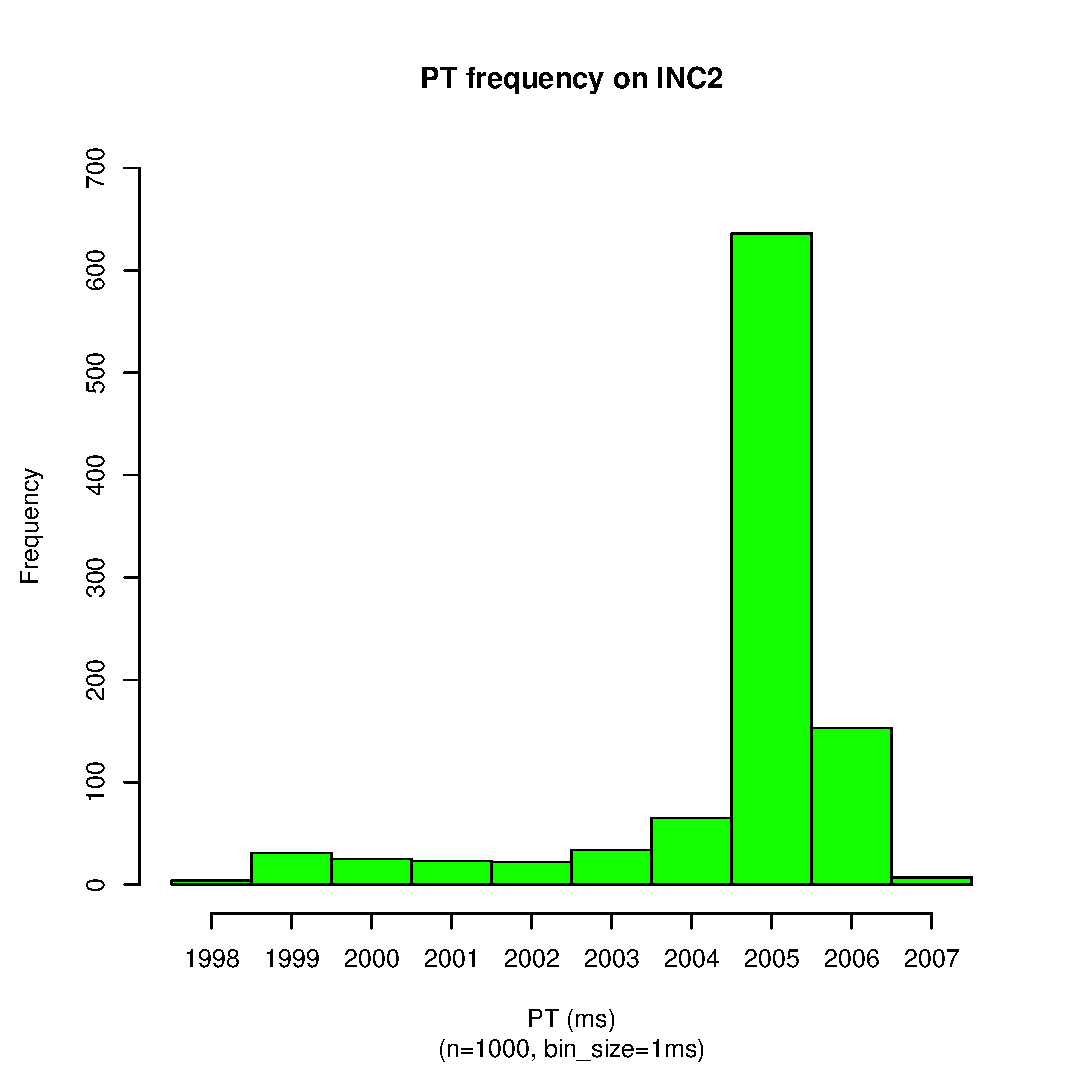
\includegraphics[scale=0.43]{repet_data1/2_sec_pt_hist_v5.eps}
		\label{fig:inc2_r1_hist_v5}
	}
	\subfigure[PT frequency on INC4]{
		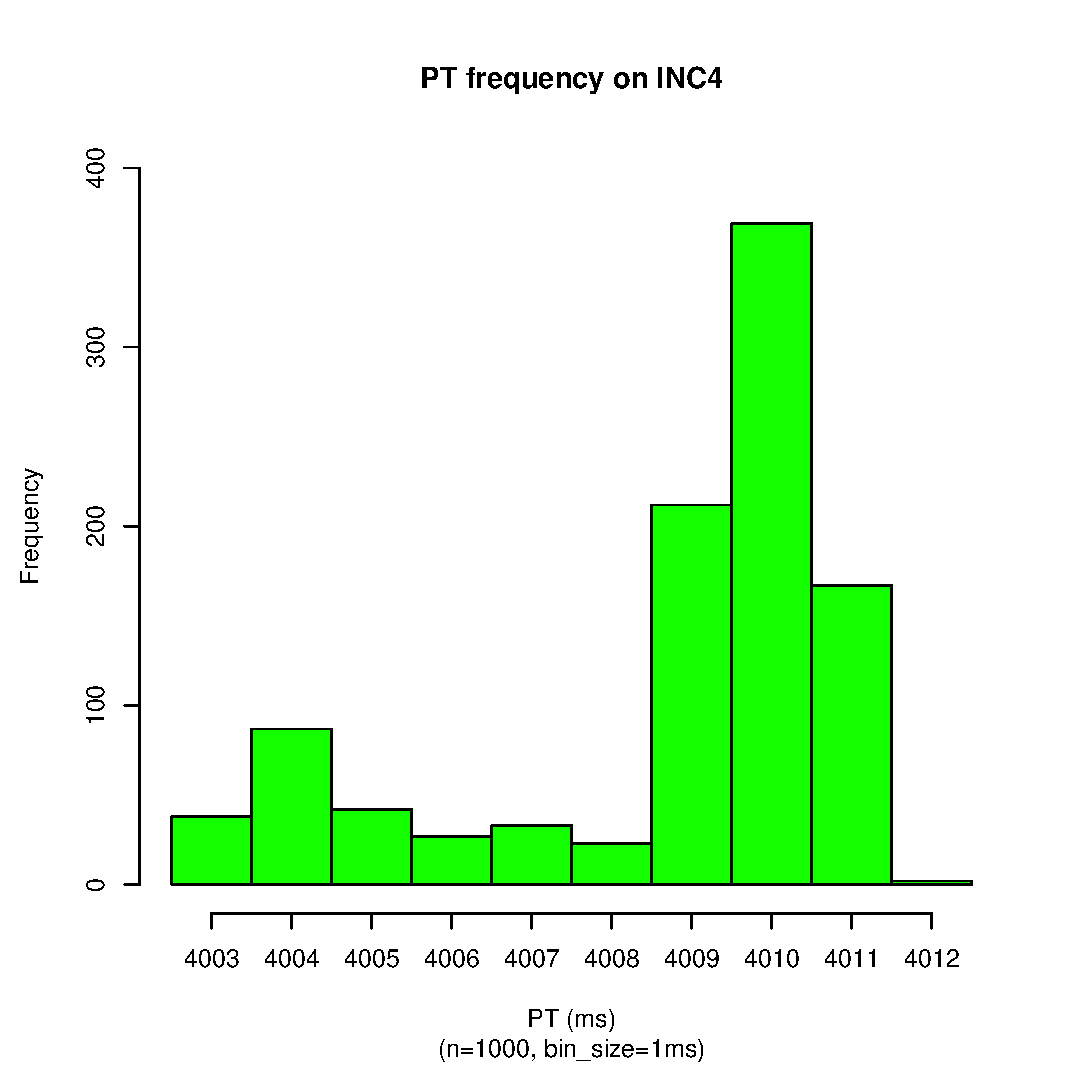
\includegraphics[scale=0.43]{repet_data1/4_sec_pt_hist_v5.eps}
		\label{fig:inc4_r1_hist_v5}
	}
	\subfigure[PT frequency on INC8]{
		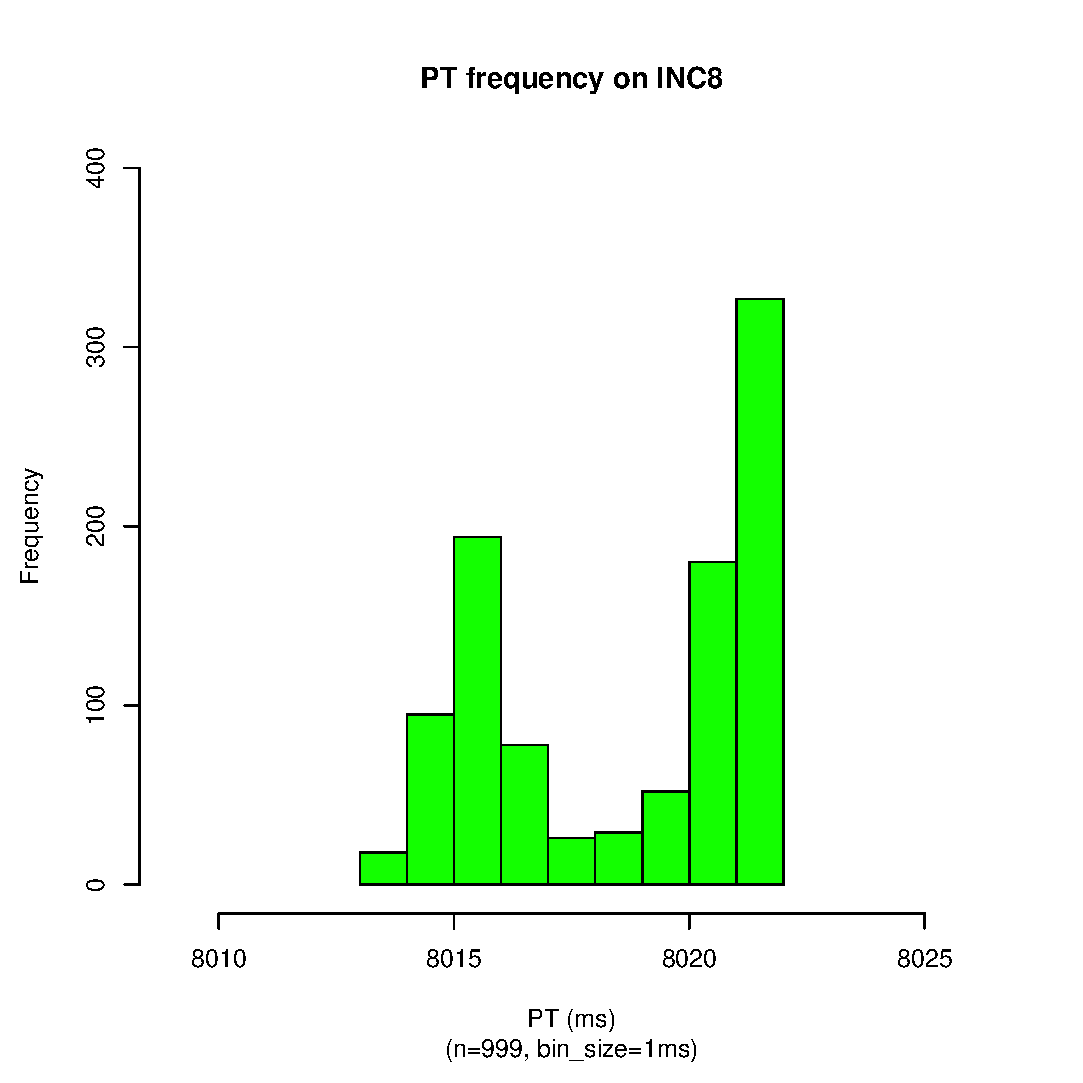
\includegraphics[scale=0.43]{repet_data1/8_sec_pt_hist_v5.eps}
		\label{fig:inc8_r1_hist_v5}
	}
	\caption{PT Histograms of INC1 ... INC8~\label{fig:s9_r1_pt_hist1}}
\end{figure}

\begin{figure}[hp!]
	\centering
	\subfigure[PT frequency on INC16]{
		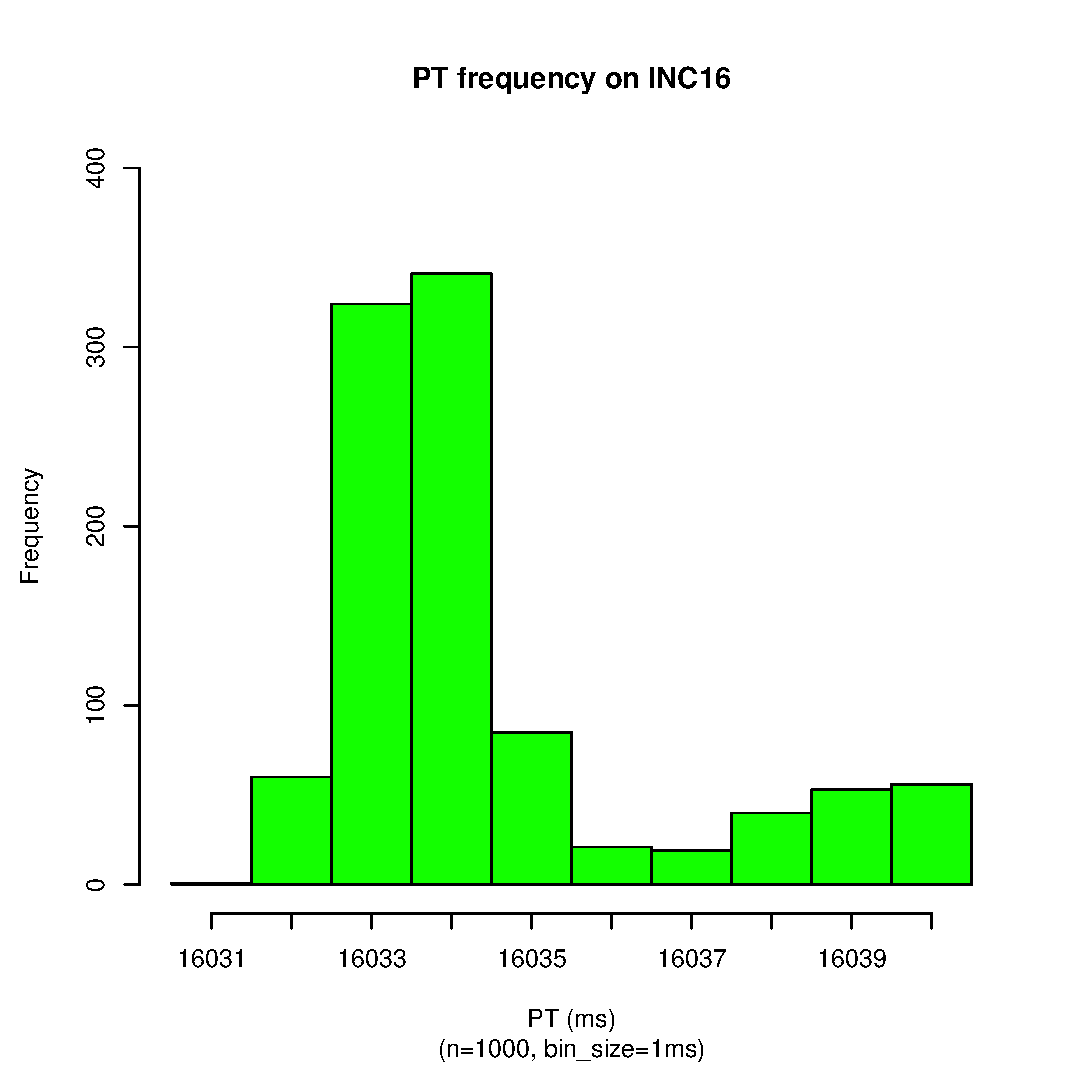
\includegraphics[scale=0.43]{repet_data1/16_sec_pt_hist_v5.eps}
		\label{fig:inc16_r1_hist_v5}
	}
	\subfigure[PT frequency on INC32]{
		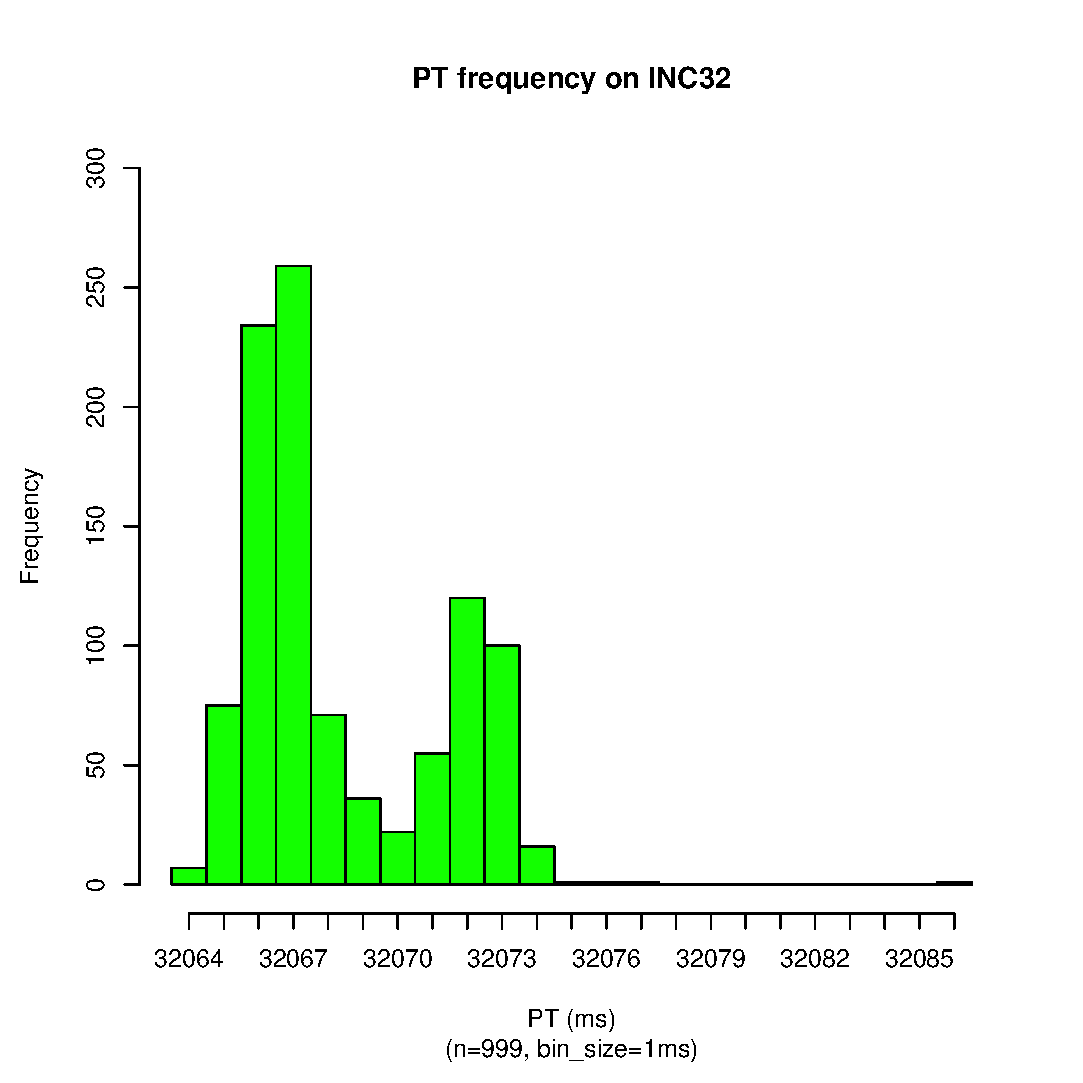
\includegraphics[scale=0.43]{repet_data1/32_sec_pt_hist_v5.eps}
		\label{fig:inc32_r1_hist_v5}
	}
	\subfigure[PT frequency on INC64]{
		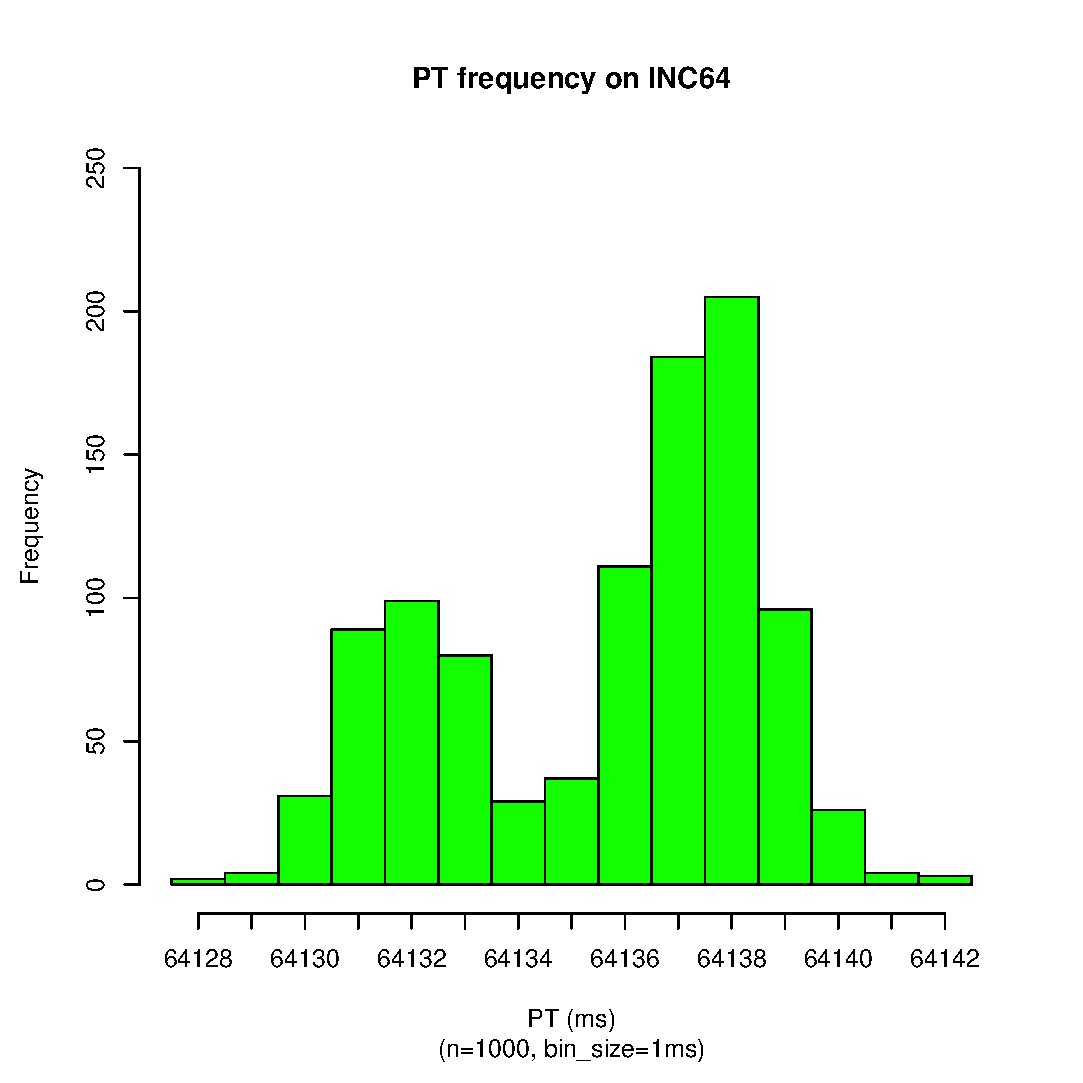
\includegraphics[scale=0.43]{repet_data1/64_sec_pt_hist_v5.eps}
		\label{fig:inc64_r1_hist_v5}
	}
	\caption{PT Histograms of INC16 ... INC64\label{fig:s9_r1_pt_hist2}}
\end{figure}

\begin{figure}[hp!]
	\centering
	\subfigure[PT frequency on INC128]{
		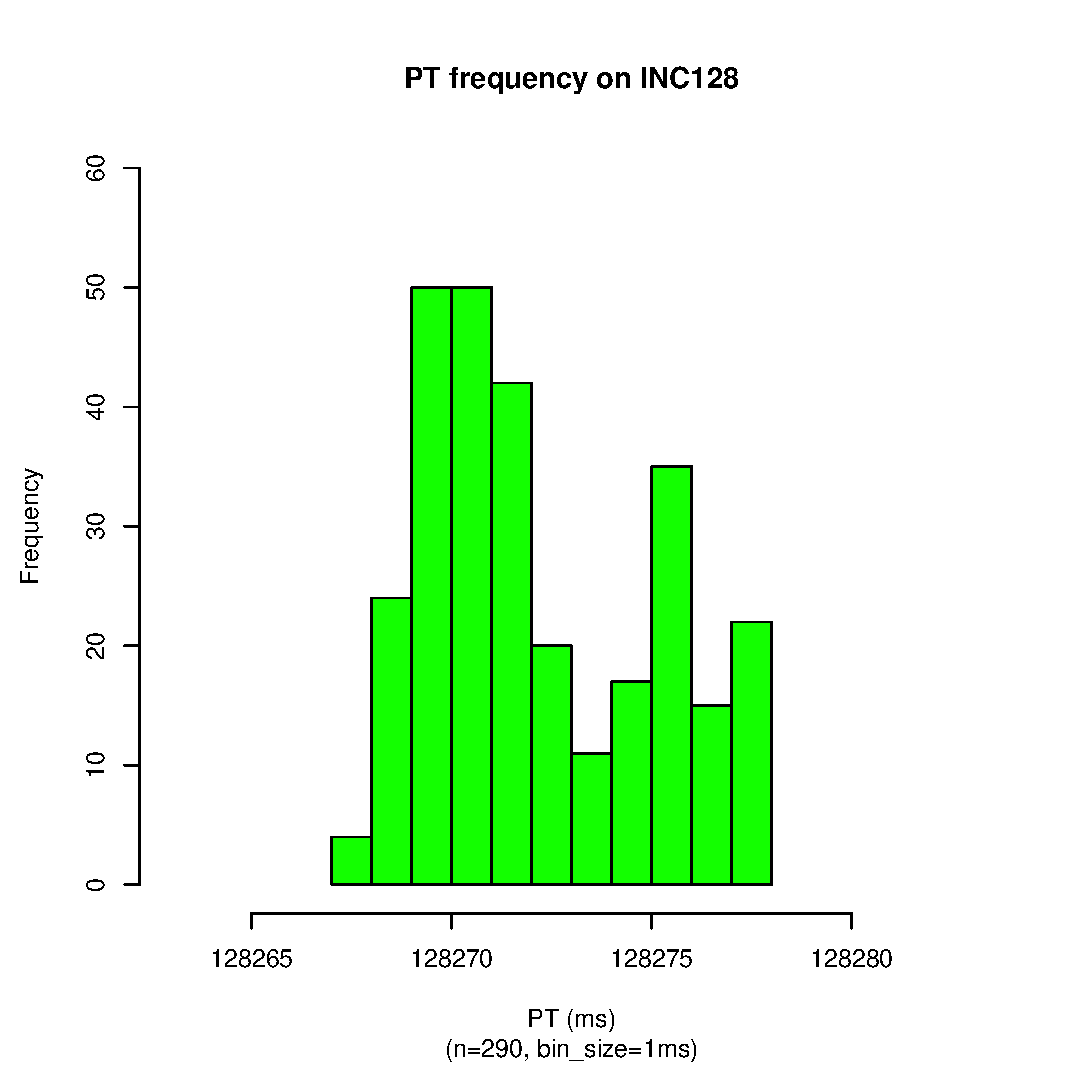
\includegraphics[scale=0.43]{repet_data1/128_sec_pt_hist_v5.eps}
		\label{fig:inc128_r1_hist_v5}
	}
	\subfigure[PT frequency on INC256]{
		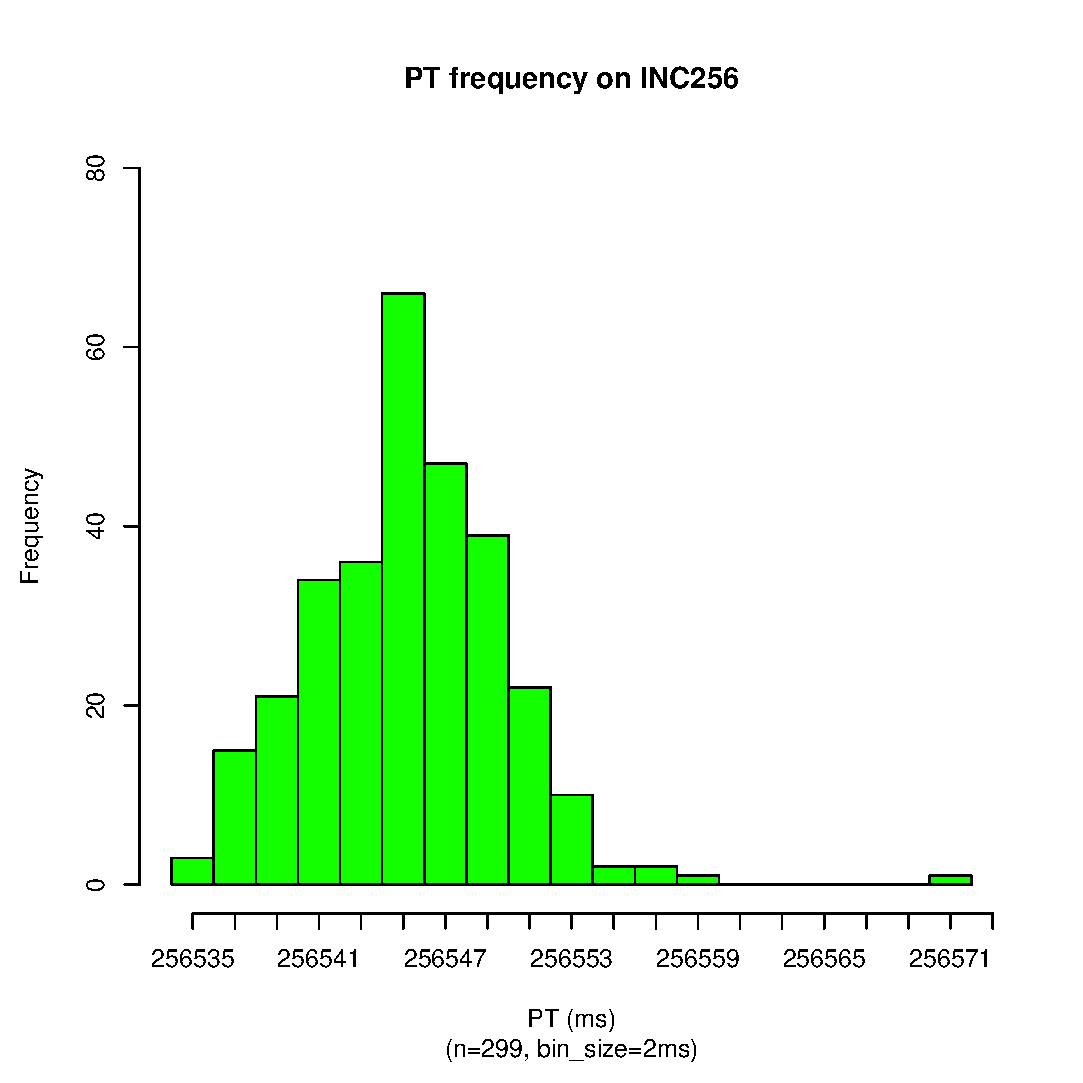
\includegraphics[scale=0.43]{repet_data1/256_sec_pt_hist_v5.eps}
		\label{fig:inc256_r1_hist_v5}
	}
	\subfigure[PT frequency on INC512]{
		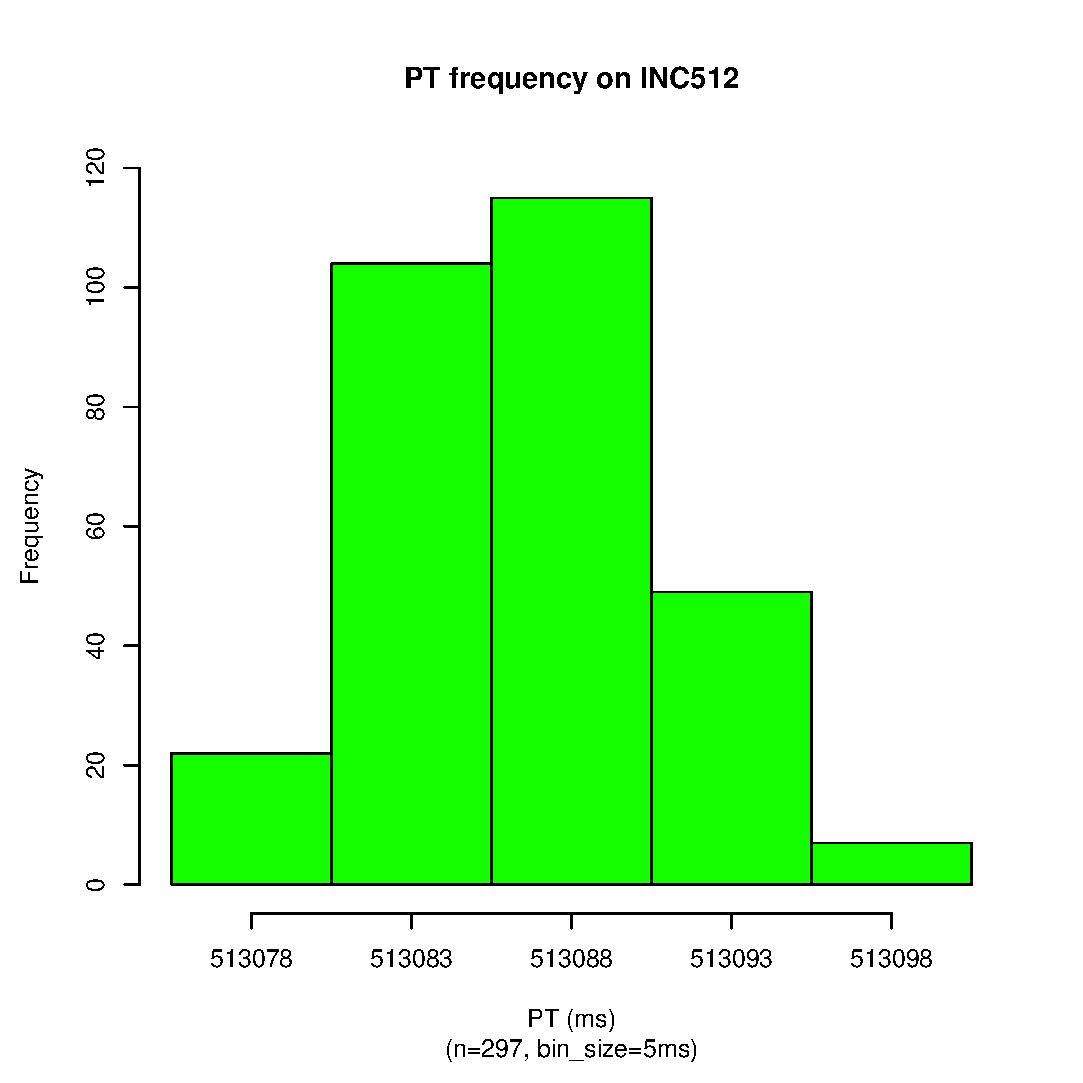
\includegraphics[scale=0.43]{repet_data1/512_sec_pt_hist_v5.eps}
		\label{fig:inc512_r1_hist_v5}
	}
	\subfigure[PT frequency on INC1024]{
		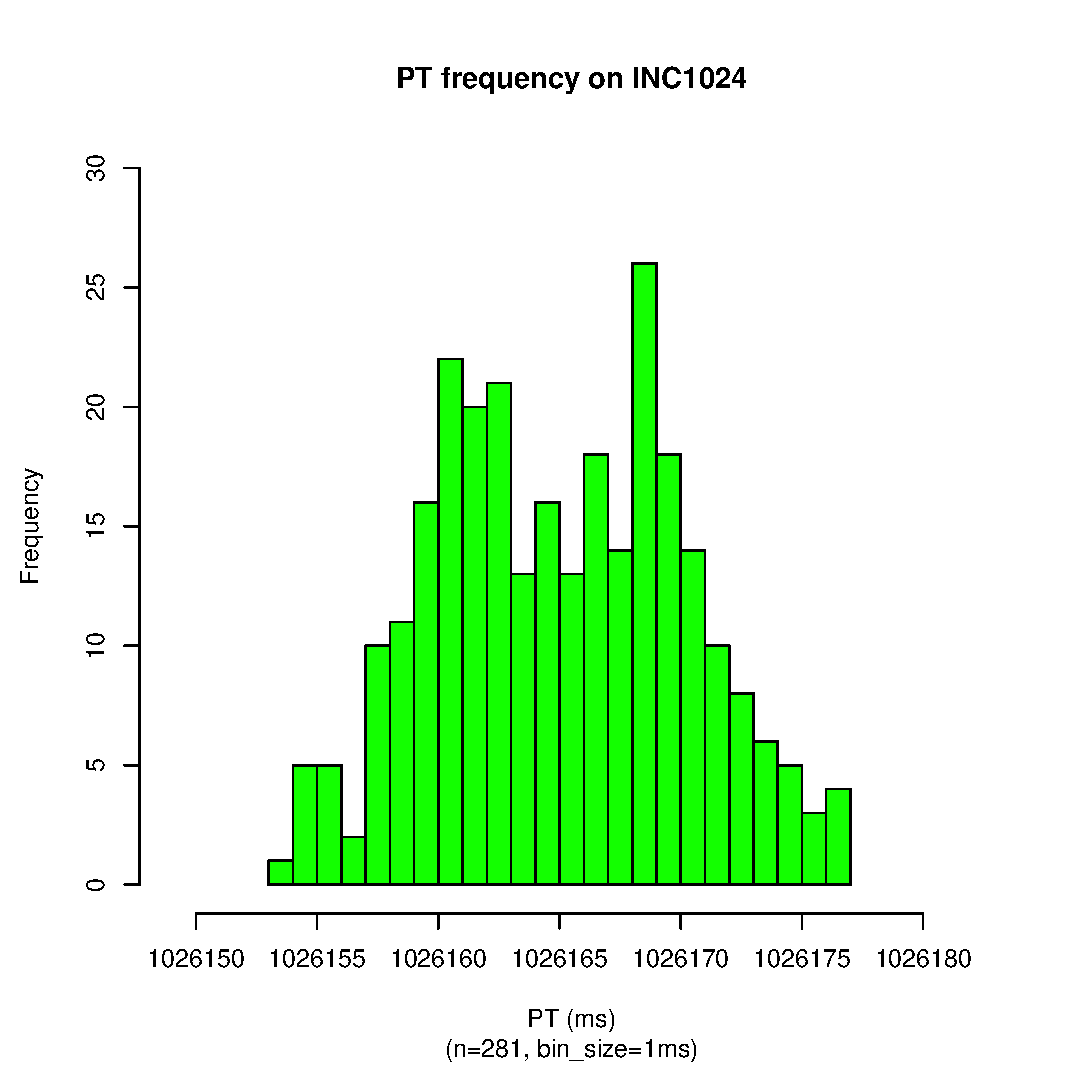
\includegraphics[scale=0.43]{repet_data1/1024_sec_pt_hist_v5.eps}
		\label{fig:inc1024_r1_hist_v5}
	}
	\caption{PT Histograms of INC256 ... INC1024~\label{fig:s9_r1_pt_hist3}}
\end{figure}

\begin{figure}[t]
	\centering
	\subfigure[PT frequency on INC2048]{
		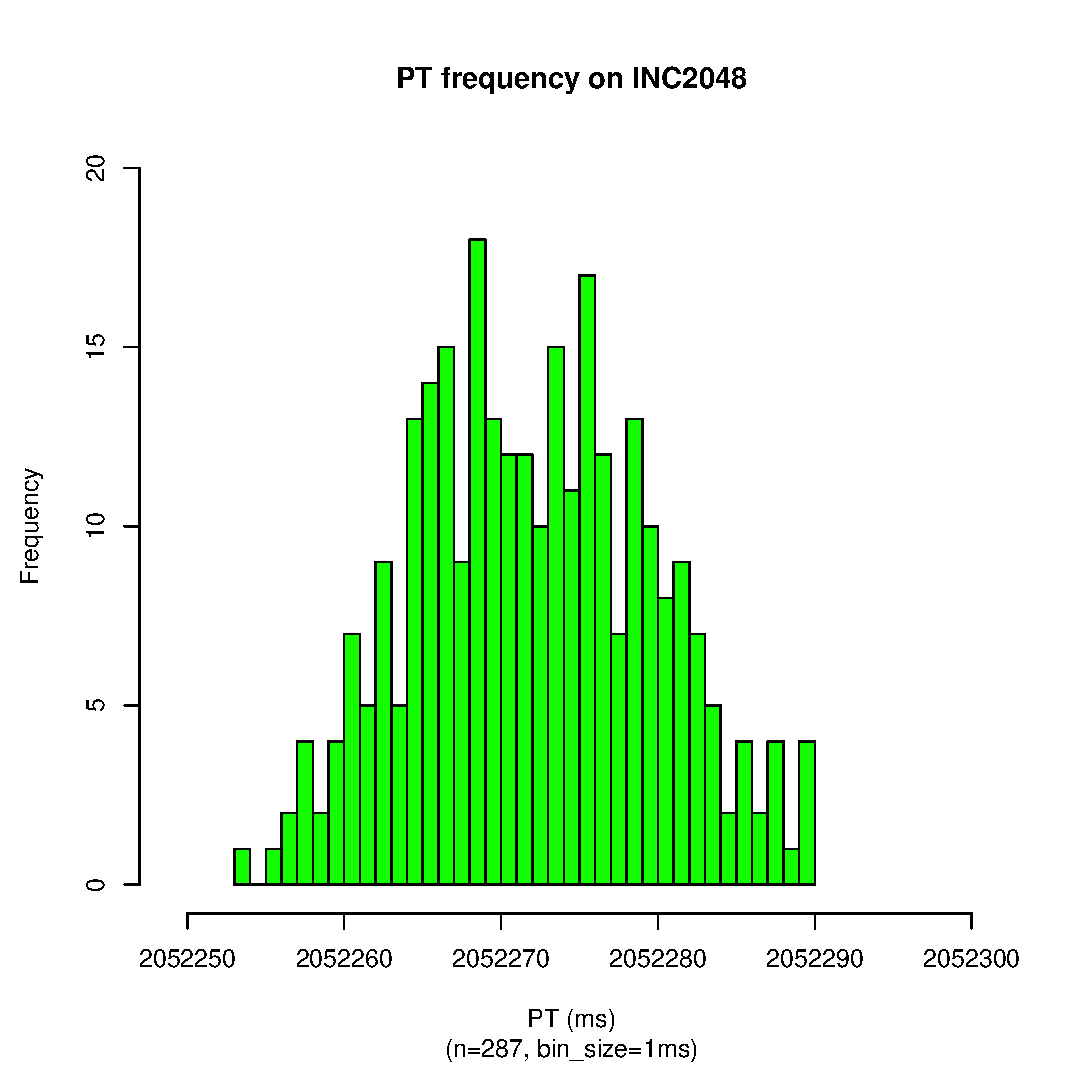
\includegraphics[scale=0.43]{repet_data1/2048_sec_pt_hist_v5.eps}
		\label{fig:inc2048_r1_hist_v5}
	}
	\subfigure[PT frequency on INC4096]{
		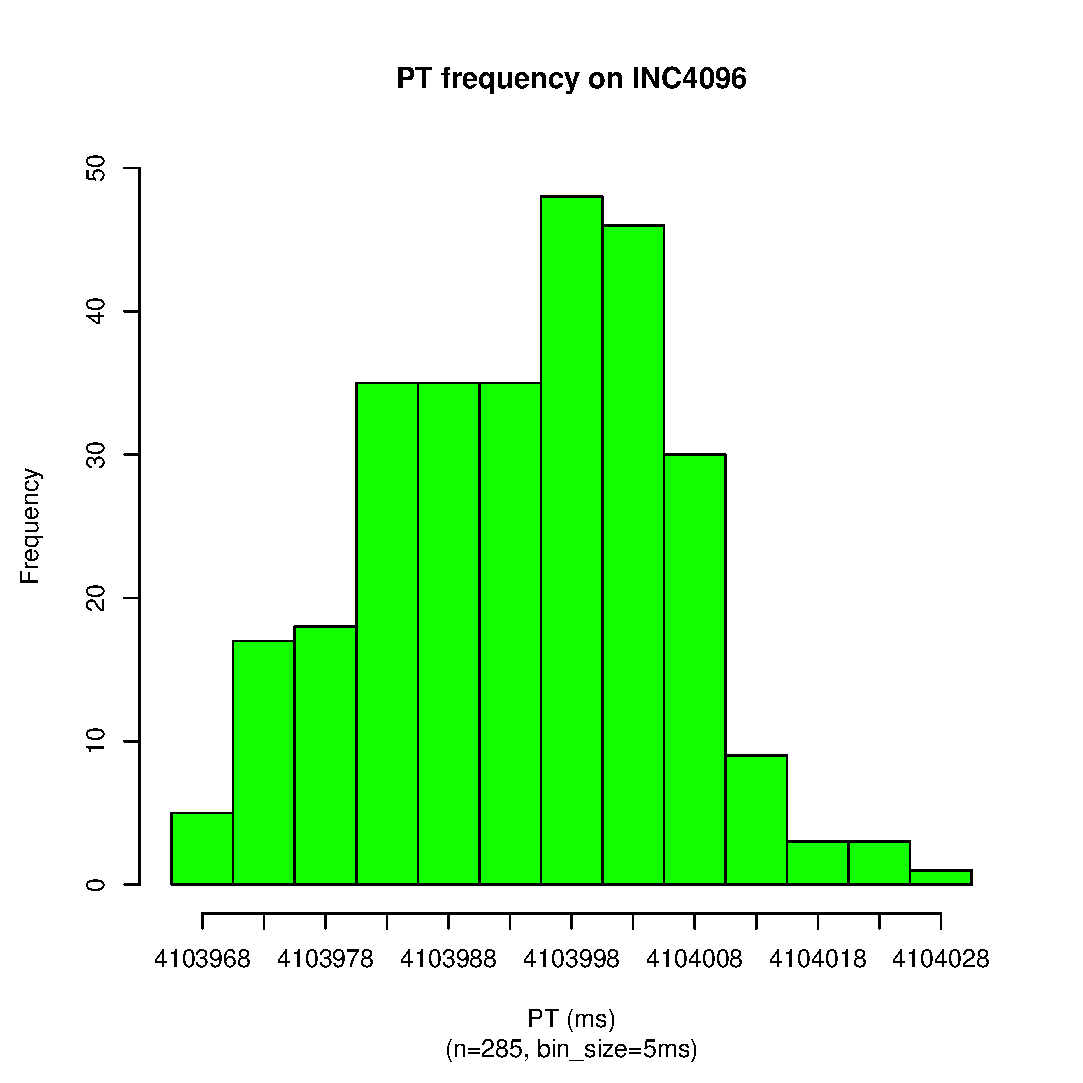
\includegraphics[scale=0.43]{repet_data1/4096_sec_pt_hist_v5.eps}
		\label{fig:inc4096_r1_hist_v5}
	}
	\caption{PT Histograms of INC2048 and INC4096~\label{fig:s9_r1_pt_hist4}}
\end{figure}

\clearpage